


\chapter{Control}

\section{Cose dette da Rizzo che non ho capito che c'entrano}\label{appendix:decentralized_joint_control_velocity_controlled}

Come accennato in precedenza, in questo caso andremo a controllare gli attuatori in velocità.
È possibile dimostrare (vedi dopo) la seguente assunzione:
$$
\mathbf{G}_v\mathbf{v}_c \approx \mathbf{K}_\omega\mathbf{K}_r\mathbf{\dot{q}}
$$
L'importante di questa espressione è la proporzionalità fra $\mathbf{G}_v$ e  $\dot{\mathbf{q}}$ (velocità), che notiamo essere indipendente dai parametri del manipolatore. Inoltre questa proporzione è tanto più valida quanto velocità/accellerazioni sono piccole (per questa cosa viene in aiuto anche il gear-reduction ratio $K_r$).

\begin{mdframed}[leftmargin=15pt, rightmargin=15pt, leftline=false, rightline=false]
	\textit{Dim.}
	
	\textit{
		Partendo dal modello dinamico {\boldmath$B(q)\ddot{q} + C(q, \dot{q})\dot{q} + F_v\dot{q} + g(q) = \tau$} introduciamo in esso la frizione viscosa elettrica. Ovvero poniamo {\boldmath$F_v = F_\text{v. mech.} + F_\text{v. electr.} = F_\text{v. mech.} + K_rK_tR_a^{-1}K_\omega K_r$}. \\
		Inoltre dal modello del motore: 
		{\boldmath$\tau_m = K_r^{-1} \tau = K_t I_a \implies \tau = K_r K_t I_a$}. Sappiamo anche che $V = Ri \implies i = \frac{V}{R}$ e quindi, ricordando che {\boldmath$V_c = G_v V_c^{'}$}, otteniamo {\boldmath $I_a = R_a^{-1}G_v V_c$}. Unendo il tutto otteniamo {\boldmath $\tau = K_r K_t R_a^{-1}G_v V_c$}.\\
		Inserendo tutto nella formula del modello dinamico otteniamo:
		\boldmath
		$$
		B(q)\ddot{q} + C(q, \dot{q})\dot{q} + F_{\text{v. mech.}}\dot{q} + g(q) = K_r K_t R_a^{-1}G_v V_c - K_rK_tR_a^{-1}K_\omega K_r
		$$
		Ovvero, raccogliendo i termini a destra (ricordando che originalmente quello era $\tau$):
		\begin{equation}\label{eq:torque_command}
			\tau =  K_r K_t R_a^{-1}(G_v V_c - K_\omega K_r \dot{q})
		\end{equation}
		Quello che otteniamo fra le parentesi è l'espressione ipotizzata inizialmente.\\
		(la quasi uguaglianza viene dal fatto che $K_r \gg 1$, $R_a$ molto piccolo, $\tau$ non troppo grosso).
	}
	
	\raggedleft $\square$
\end{mdframed}












\section{Derivazione del valore di steady-state per il motore velocity-generator}\label{appendix:torque_controlled_steady_state_derivation}


\begin{figure}[H]
	\centering
	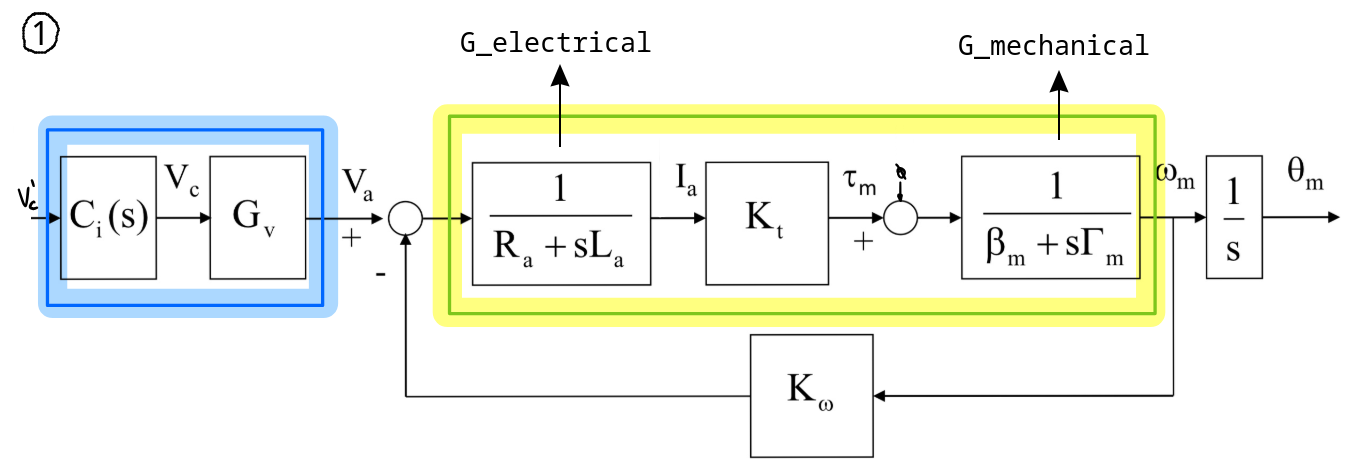
\includegraphics[width=0.7\linewidth]{images/appendix_steady_state_1}
	\label{fig:appendixsteadystate1}
\end{figure}

\begin{figure}[H]
	\centering
	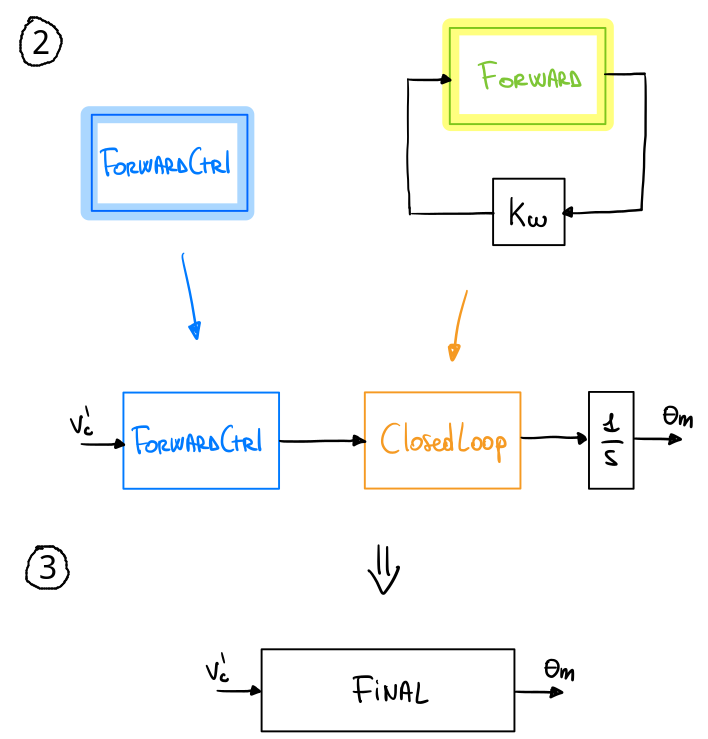
\includegraphics[width=0.6\linewidth]{images/appendix_steady_state_2}
	\label{fig:appendixsteadystate2}
\end{figure}

Per calcolare il valore di steady-state utilizziamo il tool simbolico di Matlab.\\

\circled{1} Iniziamo definendo i vari simboli e i vari blocchi:

\begin{lstlisting}[frame=single,style=Matlab-editor]
	syms s R L beta Gamma K_omega K_i G_v C_i K_t
	
	% Electrical and Mechanical balance t.f.
	G_electrical = 1/(R + s*L);
	G_mechanical = 1/(beta + s*Gamma);
\end{lstlisting}

\circled{2} Proseguiamo accorpando i percorsi di \textit{forward} e di \textit{feedback}:

\begin{lstlisting}[frame=single,style=Matlab-editor]	
% Simplify controller (remember that here K_i = 0)
ForwardCtrl = C_i * G_v;
	
% Calculate the closed-loop t.f. (supposing tau_r = 0)
Forward = G_electrical * K_t * G_mechanical;
ClosedLoop = Forward/(1 + Forward*K_omega);
\end{lstlisting}

%\begin{figure}[H]
%	\centering
%	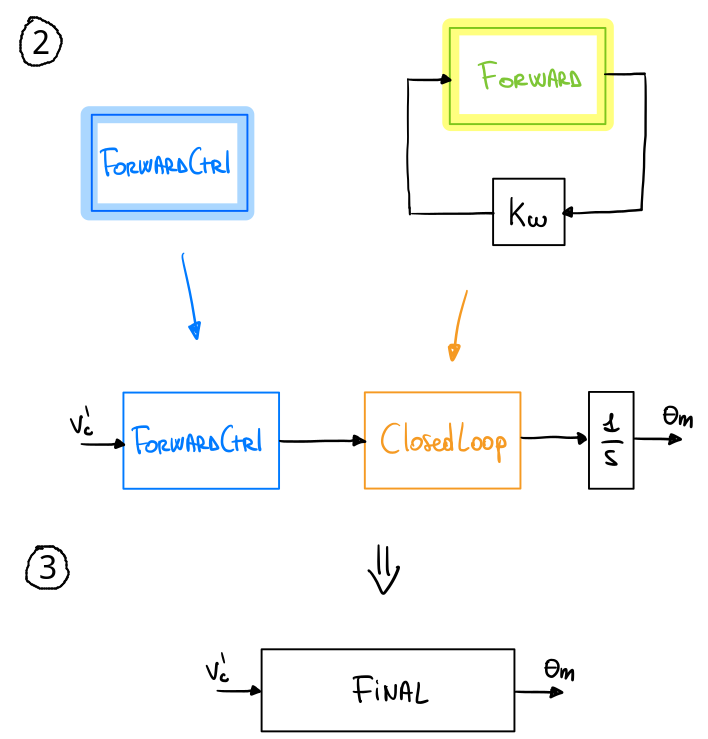
\includegraphics[width=0.6\linewidth]{images/appendix_steady_state_2}
%	\label{fig:appendixsteadystate2}
%\end{figure}


\circled{3} Infine uniamo tutto e calcoliamo il valore in \textit{steady-state} tramite il teorema del valore finale $y_\infty = \lim_{s\to0}sF(s)$:
\begin{lstlisting}[frame=single,style=Matlab-editor]
% Put everything toghether
Final = simplify(ForwardCtrl*ClosedLoop*(1/s));

% Calculate steady-state (lim_{s->0} sF(s))
steady_state = subs(s*Final, s, 0);
% Remove beta from the assumption that beta << (K_omega*K_t)/R
steady_state = subs(steady_state, beta, 0);
% Set C_i = 1
steady_state = subs(steady_state, C_i, 1);

pretty(simplify(steady_state))
\end{lstlisting}

dove, l'ultima espressione ritorna proprio:
$$
\frac{G_v}{K_\omega}
$$
$\hfill \square$